\chapter{\textbf{European Central Bank Speeches: A Case Study}}

Given the need to corroborate and expand research in the area of sentiment analysis applied to the economic sciences -- and based on the examples already observed in chapter \ref{chapter:lit}, an application in a case study is proposed here.\\

% In order to add something relevant to the literature, the proposed exercises work fundamentally with observable European economic variables\footnote{it is also worth mentioning the inclusion of the output gap, obtained from the Hodrick–Prescott filter \citep{hodrick1997postwar}}: -- with the exception of the proposed sentiment index (bag of words), made from two lexicons (VADER and LM-SA)

\section{Problem and Data Description}

Following the example of \cite{shapiro2020measuring}, \cite{barsky2012information} and \cite{shapiro2020measuring}, two practical exercises are proposed.\\

Firstly, in order to understand whether a sentiment index can be used for forecasting and estimating economic variables, and following the example of \cite{shapiro2020measuring}, we propose the estimation of two LASSO models (L1 norm) in order to identify possible relevant variables in scenarios macroeconomic models -- the first model is the conventional LASSO and the second the Adaptive LASSO. Still, in order to expand the field of estimations, an elastic net model is estimated, in order to capture improvements in model specifications and improve the selection of variables when the coefficients are close to zero  when:the coefficients are close to zero, elastic net tries to take advantage of the information provided by the variables without necessarily forcing the coefficients to zero, and without considering a scenario where all variables are used in order to improve a model (L2 norm).\\

From there, the estimation of an autoregressive vector (VAR) is considered, also following the indications of the literature \citep{shapiro2020measuring, barsky2012information} to better understand how a sentiment index relates to a macroeconomic scenario (and its variables). For this, the main focus of the second exercise is the exploration of impulse and response functions obtained through VAR.

The proposed exercises work fundamentally with observable European economic variables\footnote{it is also worth mentioning the inclusion of the output gap, obtained from the Hodrick–Prescott filter \citep{hodrick1997postwar}}, with the exception of the proposed sentiment index (bag of words), made from two lexicons (VADER and LM-SA).\\

The other series used for the exercises were obtained from the website of FRED - Federal Reserve Bank of St. Louis - and they are: Consumer Price Index: Harmonized Prices: Total All Items for the Euro Area; Consumer Opinion Surveys: Consumer Prices: Future Tendency of Inflation: European Commission and National Indicators for the Euro Area\footnote{Following the guidance of \cite{shapiro2020measuring}}; Real Gross Domestic Product (Euro/ECU series) for Euro area; Long-Term Government Bond Yields: 10-year: Main (Including Benchmark) for the Euro Area; Harmonized Unemployment Rate: Total: All Persons for the Euro Area. Two dummies were also included in the exercise, the first referring to the Subprime mortgage crisis; and the second referring to the economic crisis generated by the COVID-19 pandemic.\\

%\subsection{Sentiment Indexes}

Given that both series referring to sentiment indices are also not observable, they were obtained as proxies for the speeches of the European central bank\footnote{Speeches are available at https://www.ecb.europa.eu/press/key/date/html/index.en.html}. The methodology discussed here is based on \cite{loughran2011liability}, taking into account its contribution to the literature when referring to the applicability of sentiment analysis applied to economics.\\

According to \cite[p. 35]{loughran2011liability} it is possible to measure, as well as classify an economic text from the negative words in a way that the tone of these presents a correlation with economic and financial variables, since ``The results to date indicate that negative word classifications can be effective in measuring tone, as reflected by significant correlations with other financial variables''\\

As stated by \cite[p. 13]{shapiro2021taking} ``There is a large and growing literature aimed at quantifying sentiment from text. We use a method known as the `Bag of Words' or `lexical' approach, which relies on predefined dictionaries of words that are associated with particular sentiments'' -- in this work we also consider the polarity when taking into account the VADER -- analysis from valence, given a score. Unlike VADER, where the polarity is displayed\footnote{The polarity was obtained from the Natural Language Toolkit \cite[]{bird2009natural} module for Python from positive, negative, neutral and compound words.} the polarity of each text taking into account the LM-SA-2020 and extracting the composition of negative words in order to consider the weight of each term as a function of the total terms:

\begin{quote}
``In the context of information retrieval [\dots] note that term weighting `has an enormous impact on the effectiveness of a retrieval system.' Essentially, term weighting acknowledges that raw word counts are not the
best measure of a word’s information content''\cite[p. 42]{shapiro2020measuring}  
\end{quote}
So, given the occurrence of a negative word $W_{Negative}$, its frequency is computed so that the index, based on the negative terms, is given by:
\begin{align*}
I_{Negative, i} = \frac{W_{Negative, i}}{W_{Total, i}} \quad ,
\end{align*}

Where, $I_{Negative, i}$ represents the index score given the discourse $i$ of the corpus; $W_{Negative, i}$ represents the number of negative words given the speech $i$ of the corpus; and $W_{Total, i}$ represents the total number of words (positive, negative and neutral) given the speech $i$ of the corpus. As the European central bank usually carries out more than one speech per month and the objective is the value of the monthly index, it was necessary to group the values obtained per speech around its monthly average, so that:
\begin{align*}
    I_{t} = \frac{1}{n}\sum_{i=1}^{n}I_{Negative,i} \quad
\end{align*}

That is, the monthly value of the index is given by the average of the scores of the indexes of each speech in the same month.\\

The Figure \ref{fig:correlationvaderlmsa} presents the scatter plot between the two formulated indices: VADER (valence) and LM-SA-2020 (polarity). Even though the polarity calculation methodology is different for both lexicons, the Pearson correlation coefficient between them is, as expected, positive (69.76\%).

\begin{figure}[!h]
    \centering
    \caption{Correlation between the polarities obtained from the VADER and LM-SA-2020 lexicons (negative words)}
    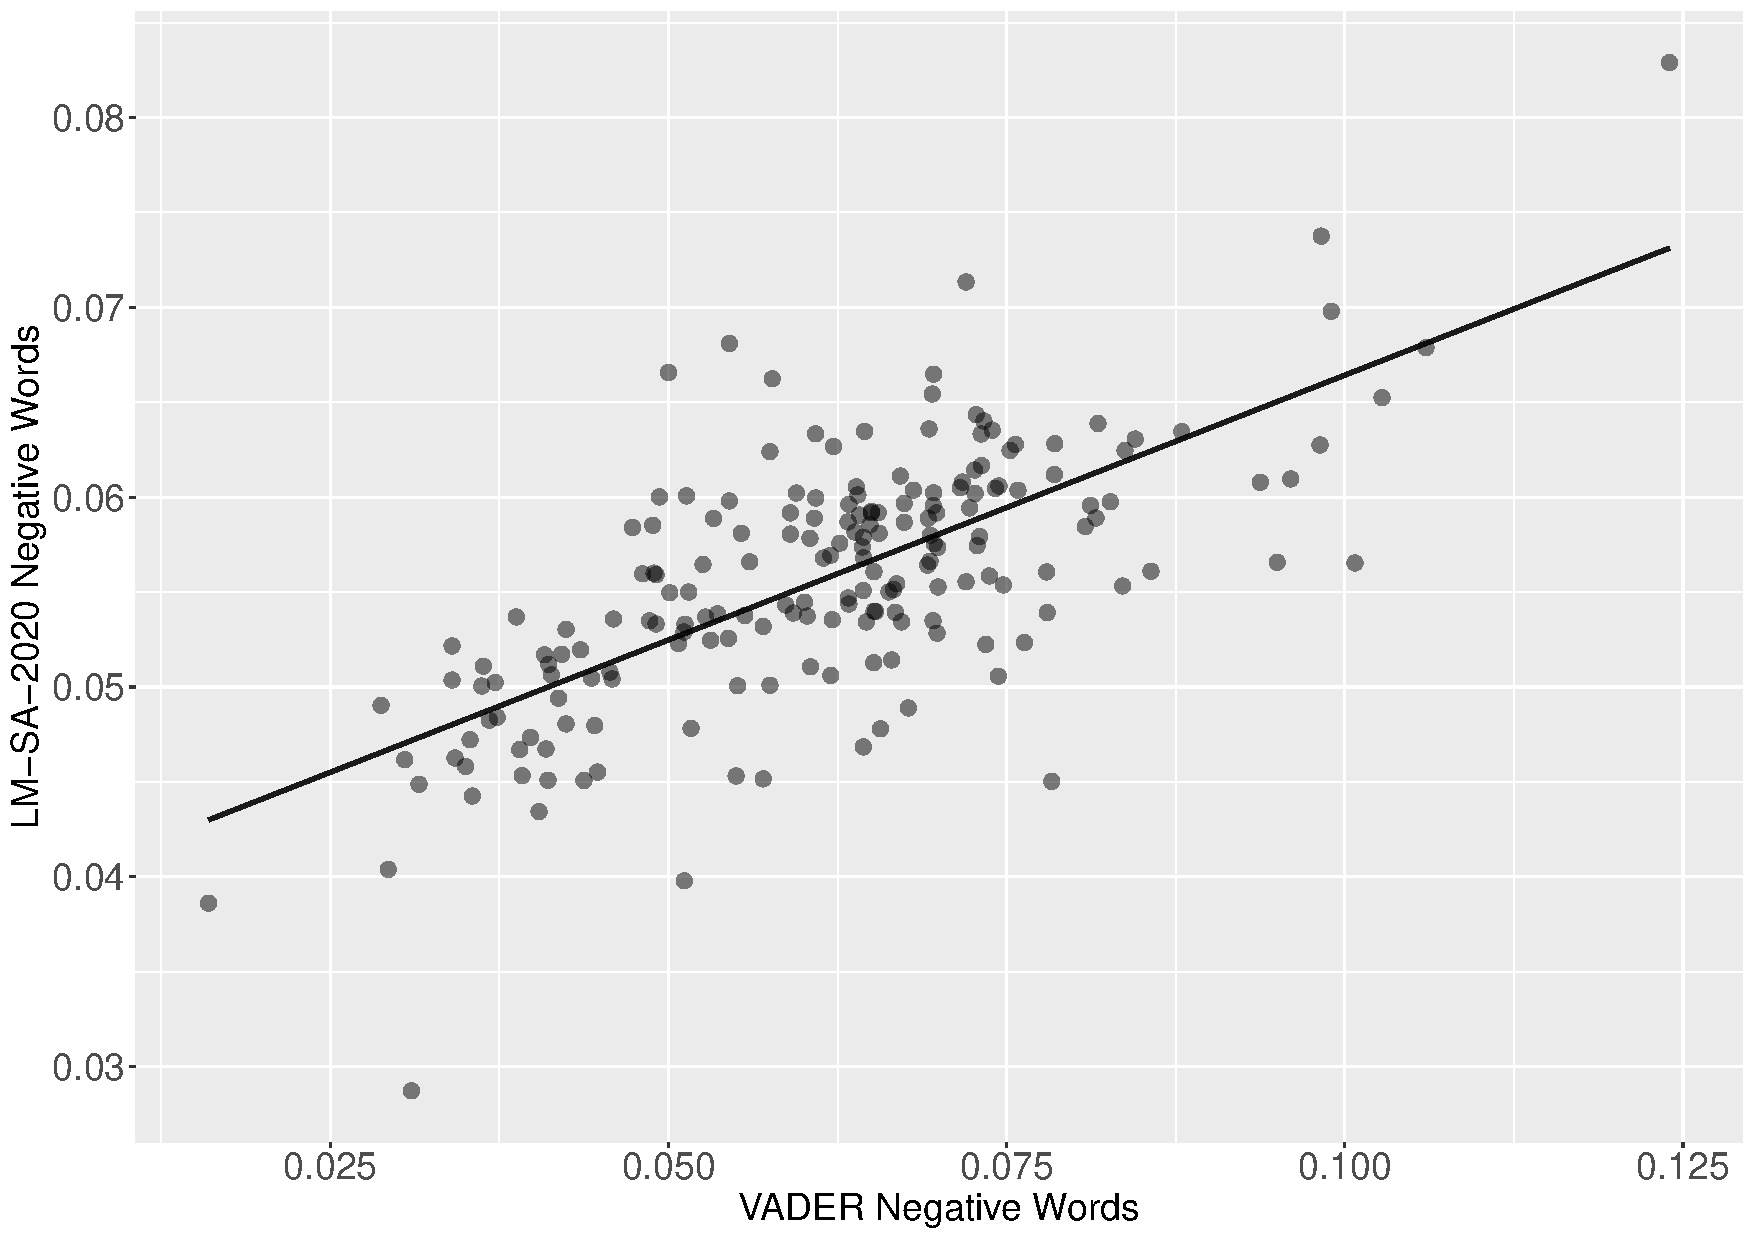
\includegraphics[width=.7\textwidth]{images/correlation_vader_lm.pdf}
    \label{fig:correlationvaderlmsa}
\end{figure}

Both indices are used in the case studies. At first, it would be recommended to \cite[p. 62]{loughran2011liability} the main use of a lexicon focused on economic and financial terms and words (LM-SA-2020) -- however, VADER is used due to the excellent results that this lexicon presents. Furthermore, it is considered an exercise to compare both lexicons: in consideration of the fact that the LM-SA-2020 focuses on economic and financial terms and words, in contrast to VADER, which, even being aimed at media analysis, has excellent results against similar lexicons.

\section{Experimental Setup}

Since the case studies consider certain statistical and econometric techniques, it is necessary to consider some assumptions in relation to the methodologies adopted and to analyze the behavior of the time series.\\

The time horizon adopted was from January 2005 to December 2020 -- it was not possible to extend this work until the year 2021 due to lack of data at the time of writing this: moreover, the choice of period was arbitrary, considering , however, the availability of the economic series and the availability of the speeches of the European Central Bank used. In all, the original database is composed of 132 observations so that two of the variables are sentiment indices (VADER and LM-SA-2020); two dummies are considered for the estimation of the variable selection models, namely: 1st- COVID, so that if the time point is February, March, or April 2020, COVID = 1, otherwise COVID = 0; 2nd - Debt Crisis in Europe, so that if the time period is from September 2011 to January 2013, the dummy assumes the value of 1, otherwise 0; all other variables are observable economic variables -- with the exception of the output gap, obtained from the Hodrick-Prescott filter.\\

In addition, it is noteworthy that, for convenience in relation to the estimations and the number of observations, it was chosen to use series of monthly frequency.\\






\subsection{Unit Root Tests}

\section{Modeling}

\begin{align} \label{eq:lasso}
    \hat{\beta}^{lasso} = \argmin_{\beta} \left\{ \sum_{i=1}^{n} \left( y_i - \sum_{j=1}^p x_{i,j}b_j \right)^2 + \lambda \sum_{j=1}^p |b_j| \right\}
\end{align}

\begin{align} \label{eq:lassoadaptive}
    \hat{\beta}^{alasso} = \argmin_{\beta} \left\{\sum_{i=1}^{n} \left( y_i - \sum_{j=1}^p x_{i,j}b_j \right)^2 + \lambda \sum_{j=1}^p |b_j| \right\}
\end{align}

According to \cite{zou2005regularization}, an elastic net estimator is given by:
\begin{align}\label{eq:elasticnet}
    \hat{\beta}^{enet} = \argmin_{\beta} \left\{ \sum_{i=1}^{n} \left( y_i - \sum_{j=1}^p x_{i,j}b_j \right)^2 + \lambda_1 \sum_{j=1}^p |b_j| + \lambda_2 \sum_{j=1}^p b_j^2 \right\}
\end{align}




%pre-processing
% cross validation

%learning algorithms
%evaluation metrics

\section{Experimental Results}






\begin{figure}
    \centering
    \caption{Impulse Response of a Sentiment Index (LM-SA) Shock on Economic Activity}
    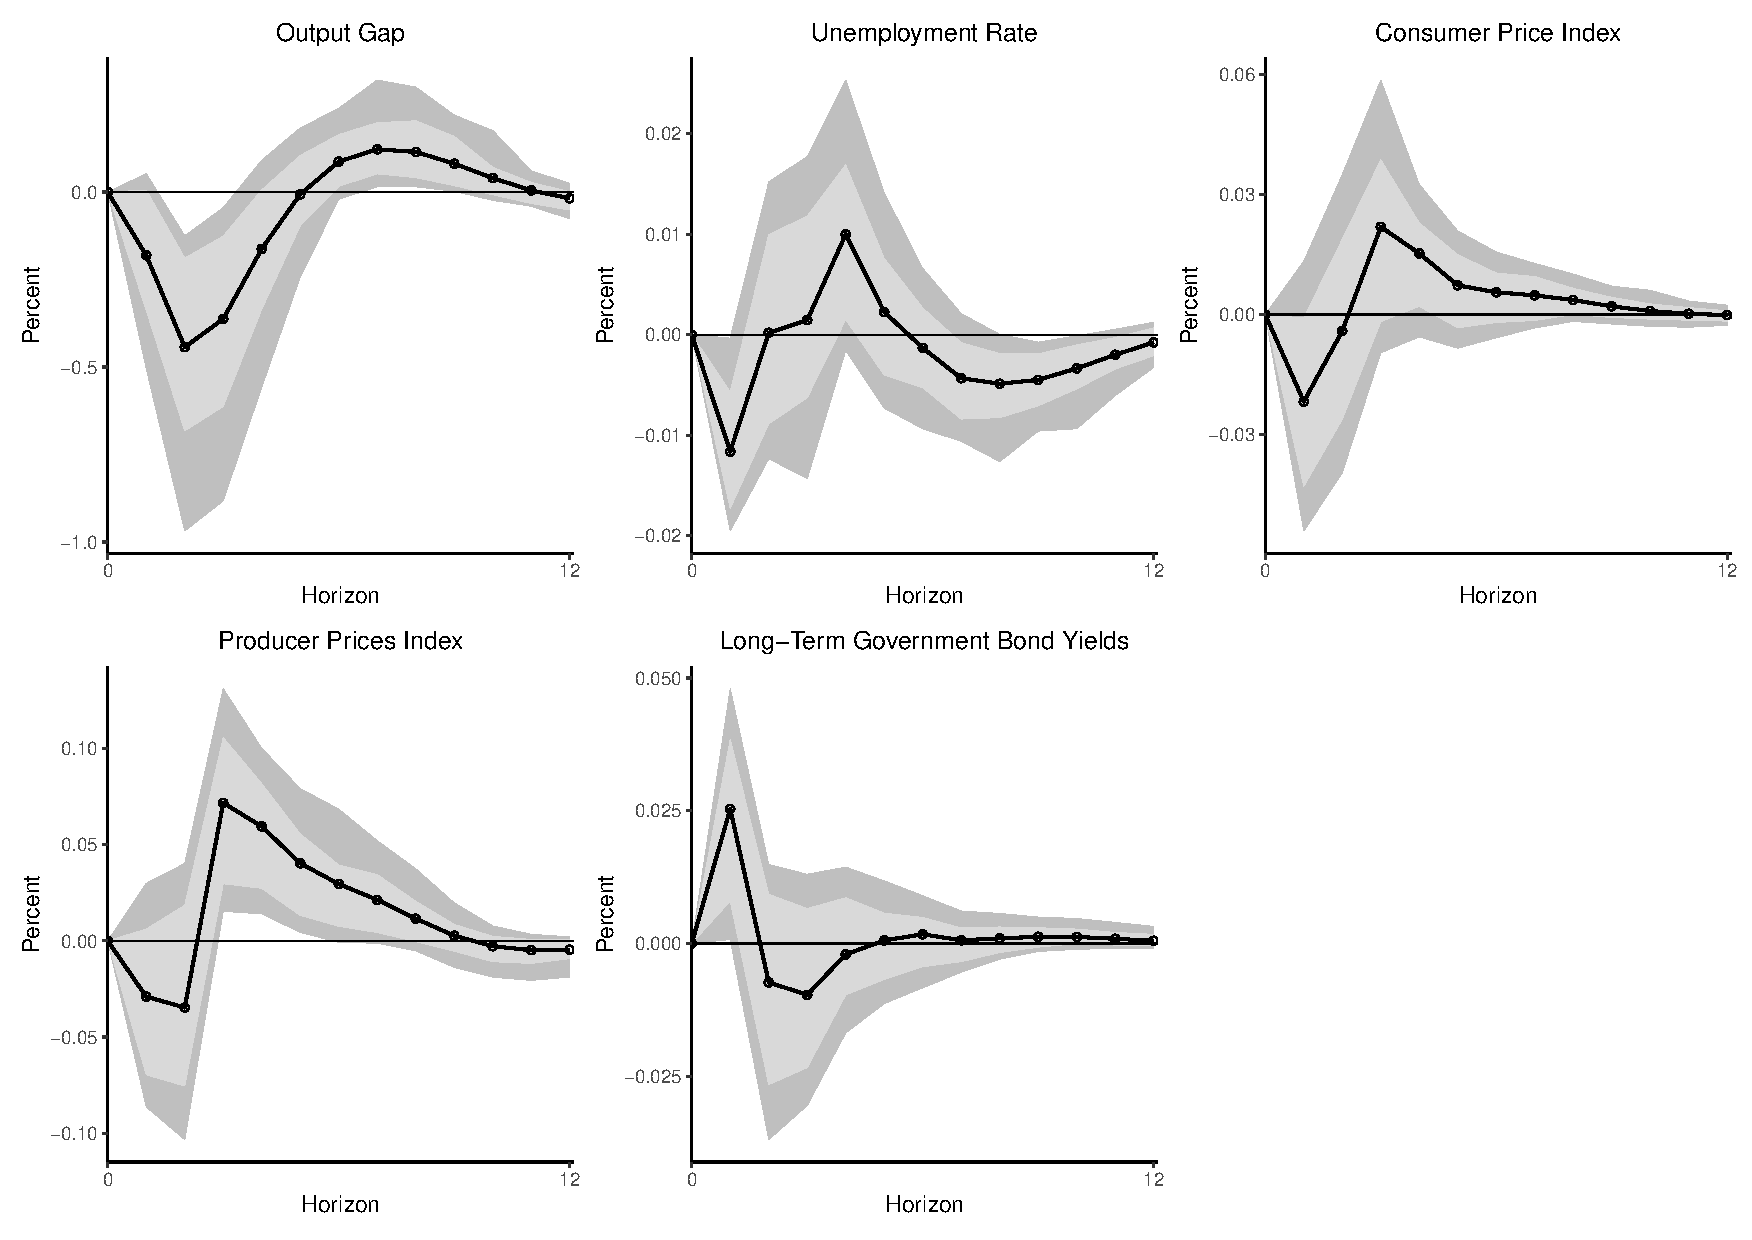
\includegraphics[width=\textwidth]{images/irf_lm.pdf}
    \caption*{Impulse Response from a sentiment index shock (LM-SA). The variables are described as follows: Output gap -- obtained from a HP filter from Real Gross Domestic Product (Euro/ECU series) for Euro area; Unemployment Rate -- Harmonized Unemployment Rate: Total: All Persons for the Euro Area}
    \label{fig:irflm}
\end{figure}


\begin{figure}
    \centering
    \caption{Impulse Response of a Sentiment Index (VADER) Shock on Economic Activity}
    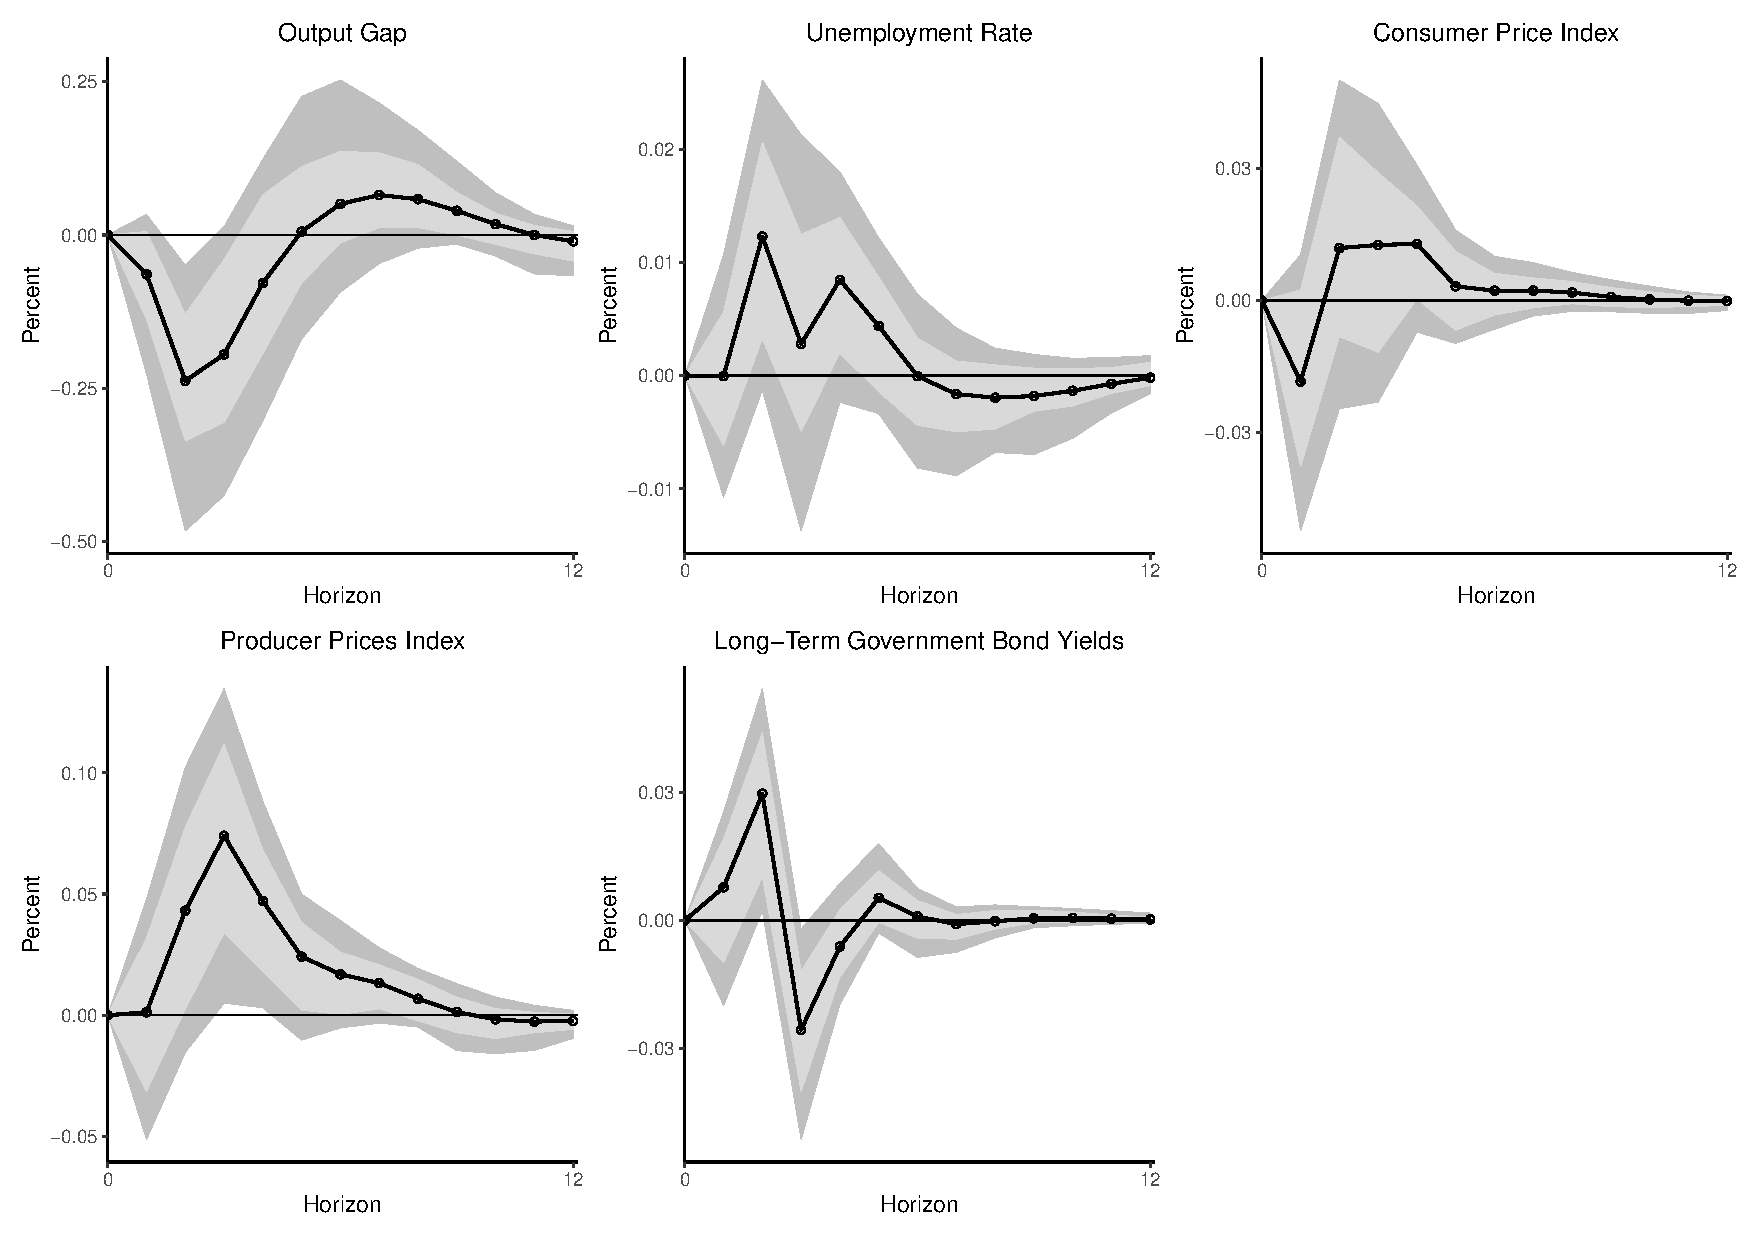
\includegraphics[width=\textwidth]{images/irf_vader.pdf}
    \caption{Caption}
    \label{fig:my_label}
\end{figure}

\section{Discussion}

\begin{landscape}


\begin{table}[]
\caption{Variable Selection Models: VADER Sentiment}
\label{tab:selectionvader}
\begin{adjustbox}{max width=\linewidth}
\begin{tabular}{llllllllll}
\hline
                         & \multicolumn{3}{c}{Consumer Opinion   Surveys} & \multicolumn{3}{c}{Unemployment Rate}      & \multicolumn{3}{c}{Interest Rate}         \\
                         & Lasso     & Adaptive Lasso    & Elastic Net    & Lasso    & Adaptive Lasso   & Elastic Net  & Lasso   & Adaptive Lasso   & Elastic Net  \\
Consumer Opinion Surveys & x         &                   & x              & x        &                  & x            & x       & x                & x            \\
Unemployment Rate        & x         & x                 & x              & x        & x                & x            & x       & x                & x            \\
Interest Rate            & x         & x                 & x              &          &                  & x            & x       & x                & x            \\
Consumer Price Index     & x         & x                 & x              & x        & x                & x            & x       & x                & x            \\
Gross Domestic Product   & x         &                   & x              &          & x                & x            & x       & x                & x            \\
Producer Prices Index    & x         & x                 & x              & x        & x                & x            & x       & x                & x            \\ \hline
VADER Sentiment          & x         & x                 & x              &          & x                & x            & x       & x                & x            \\ \hline
                         & \multicolumn{3}{c}{Consumer Price Index}       & \multicolumn{3}{c}{Gross Domestic Product} & \multicolumn{3}{c}{Producer Prices Index} \\
                         & Lasso     & Adaptive Lasso    & Elastic Net    & Lasso    & Adaptive Lasso   & Elastic Net  & Lasso   & Adaptive Lasso   & Elastic Net  \\
Consumer Opinion Surveys & x         & x                 &                & x        &                  & x            & x       & x                & x            \\
Unemployment Rate        &           &                   & x              & x        & x                & x            & x       & x                & x            \\
Interest Rate            & x         & x                 & x              & x        & x                & x            & x       & x                & x            \\
Consumer Price Index     &           &                   & x              &          & x                & x            & x       & x                & x            \\
Gross Domestic Product   &           &                   & x              &          &                  & x            & x       & x                & x            \\
Producer Prices Index    & x         & x                 & x              & x        & x                & x            & x       & x                & x            \\ \hline
VADER Sentiment          & x         & x                 & x              & x        & x                & x            & x       & x                & x \\ \hline    
\end{tabular}
\end{adjustbox}
\caption*{Note: the checkmarks symbolize that at least one of the regressors (contemporary or 12 lags) was estimated with non-zero coefficients by the LASSO, Adaptive LASSO or Elastic Net estimator indicated by the column headers. The dependent variable for each model is listed above the column headings.}
\end{table}
\end{landscape}



\begin{landscape}


\begin{table}[]
\caption{Variable Selection Models: LM-SA Sentiment}
\label{tab:selectionlm}
\begin{adjustbox}{max width=\linewidth}
\begin{tabular}{llllllllll}
\hline
                         & \multicolumn{3}{l}{Consumer Opinion Surveys} & \multicolumn{3}{l}{Unemployment Rate}      & \multicolumn{3}{l}{Interest Rate}         \\
                         & Lasso    & Adaptive Lasso    & Elastic Net   & Lasso    & Adaptive Lasso   & Elastic Net  & Lasso   & Adaptive Lasso   & Elastic Net  \\
Consumer Opinion Surveys & x        &                   & x             & x        &                  & x            & x       & x                & x            \\
Unemployment Rate        & x        & x                 & x             & x        & x                & x            & x       & x                & x            \\
Interest Rate            & x        & x                 & x             &          &                  & x            & x       & x                & x            \\
Consumer Price Index     & x        & x                 & x             &          & x                & x            & x       & x                & x            \\
Gross Domestic Product   & x        &                   & x             & x        & x                & x            & x       & x                & x            \\
Producer Prices Index    & x        & x                 & x             &          & x                & x            & x       & x                & x            \\ \hline
LM-SA Sentiment          & x        & x                 & x             & x        & x                & x            & x       & x                & x            \\ \hline
                         & \multicolumn{3}{l}{Consumer Price Index}     & \multicolumn{3}{l}{Gross Domestic Product} & \multicolumn{3}{l}{Producer Prices Index} \\
                         & Lasso    & Adaptive Lasso    & Elastic Net   & Lasso    & Adaptive Lasso   & Elastic Net  & Lasso   & Adaptive Lasso   & Elastic Net  \\
Consumer Opinion Surveys & x        & x                 & x             & x        &                  & x            & x       & x                & x            \\
Unemployment Rate        &          &                   &               & x        & x                & x            & x       & x                & x            \\
Interest Rate            & x        & x                 & x             & x        & x                & x            & x       & x                & x            \\
Consumer Price Index     &          &                   &               &          &                  & x            & x       & x                & x            \\
Gross Domestic Product   &          &                   & x             &          &                  & x            & x       & x                & x            \\
Producer Prices Index    & x        & x                 & x             & x        & x                & x            & x       & x                & x            \\ \hline
LM-SA Sentiment          & x        & x                 & x             & x        & x                & x            & x       & x                & x    \\ \hline     
\end{tabular}
\end{adjustbox}
\caption*{Note: the checkmarks symbolize that at least one of the regressors (contemporary or 12 lags) was estimated with non-zero coefficients by the LASSO, Adaptive LASSO or Elastic Net estimator indicated by the column headers. The dependent variable for each model is listed above the column headings.}
\end{table}
\end{landscape}













